



%\chapter{First appendix}
%\label{chapter:first-appendix}






%This is the first appendix. You could put some test images or verbose data in an
%appendix, if there is too much data to fit in the actual text nicely.

%For now, the Aalto logo variants are shown in Figure~\ref{fig:aaltologo}.

%\begin{figure}
%\begin{center}
%\subfigure[In %English]{
\includegraphics[width=.8\textwidth]{images/aalto-logo-en}}
%\subfigure[Suomeksi]{
\includegraphics[width=.8\textwidth]{images/aalto-logo-fi}}
%\subfigure[P� svenska]{
\includegraphics[width=.8\textwidth]{images/aalto-logo-se}}
%\caption{Aalto logo variants}
%\label{fig:aaltologo}
%\end{center}
%\end{figure}

\chapter{Augmentation using data warping}
\label{chapter:first-appendix}
\lstset{language=Python, caption=Function to create data warping, label=Simple data warping}
\begin{lstlisting}
def augmenting_f(X):
	"""Augment data by adding random slope background"""
	total_samples = X.shape[0]
	n_features = X.shape[1]
	
	xs = np.linspace(0, 1, n_features)
	xs = np.tile(xs, (total_samples, 1))
	
	# expand and transpose so that numpy broacasting multiplies each
	# row in the features by one slope
	slopes = np.random.normal(0, 0.03/2.355, total_samples)
	slopes = np.expand_dims(slopes, axis=0).T
	X += xs*slopes
	
	return X
\end{lstlisting}

\chapter{Augmentation using SMOTE}
\label{chapter:second-appendix}
\lstset{language=Python, caption=Implimentation of SMOTE, label=Simple data augmentation}
\begin{lstlisting}

from imblearn.over_sampling import SMOTE, ADASYN

augmented_x, augmented_y = SMOTE(random_state=123).fit_sample(origina_x, original_y)

\end{lstlisting}

\chapter{Augmentation using GANs}
\label{chapter:third-appendix}
\lstset{language=Python, caption=Implimentation of GANs,label=GAN}


\begin{lstlisting}

class GAN():
	def __init__(self,train_data,rand_dim,dense_unit,batch_size,
	log_interval=500):

	self.train = train_data
	self.rand_dim = rand_dim
	self.data_dim = train_data.shape[1]
	self.dense_unit = dense_unit 
	self.batch_size = batch_size
	#self.nb_steps = nb_steps
	self.log_interval=log_interval
	self.disc_loss_real = []
	self.disc_loss_generated = []
	self.combined_loss = []
	
	
	
	optimizer = keras.optimizers.Adam(lr= 5e-4, beta_1=0.5, beta_2=0.9)
	
	# Build and compile the discriminator
	self.discriminator = self.build_discriminator()
	self.discriminator.compile(optimizer=optimizer, loss='binary_crossentropy')
	
	# Build and compile the generator
	self.generator = self.build_generator()
	self.generator.compile(optimizer=optimizer, loss='binary_crossentropy')
	
	# The generator takes noise and input
	z = keras.Input(shape=(rand_dim,))
	#gen = self.generator(z)
	
	# For the combined model we will only train generator
	self.discriminator.trainable = False
	
	# Discriminator takes generated image as input and checks its validity
	dis = self.discriminator(self.generator(z))
	
	# The combined model = generator + discriminator tkaes
	# noise as input => generated images => determines validity
	self.combined = keras.models.Model(z,dis)
	self.combined.compile(optimizer=optimizer, loss='binary_crossentropy')
	
	def build_generator(self):
	generator_input = layers.Input(shape=(self.rand_dim, ))
	x = layers.Dense(self.dense_unit, activation='relu')(generator_input)
	x = layers.Dense(self.dense_unit*2, activation='relu')(x)
	x = layers.Dense(self.dense_unit*4, activation='relu')(x)
	x = layers.Dense(self.data_dim)(x)    
	generator_model = models.Model(inputs=[generator_input],
	outputs=[x],name='generator')
	return generator_model
	
	def build_discriminator(self):
	discriminator_input = layers.Input(shape=(self.data_dim,))
	x = layers.Reshape((-1, 1))(discriminator_input)
	x = layers.Conv1D(100, 20, activation='relu')(x)
	x = layers.Dropout(0.2)(x)
	x = layers.Flatten()(x)
	
	x = layers.Dense(self.dense_unit*4, activation='relu')(x)
	# x = layers.Dropout(0.1)(x)
	x = layers.Dense(self.dense_unit*2, activation='relu')(x)
	# x = layers.Dropout(0.1)(x)
	x = layers.Dense(self.dense_unit, activation='relu')(x)
	x = layers.Dense(1, activation='sigmoid')(x)
	# x = layers.Dense(1)(x)
	
	generator_model= models.Model(inputs=[discriminator_input],outputs=[x],
	name='discriminator')
	return generator_model
	
	
	def get_data_batch(self,seed):
	
	# iterate through shuffled indices, so every sample gets covered evenly
	start_i = (self.batch_size * seed) % (self.train.shape[0])
	stop_i = start_i + self.batch_size
	shuffle_seed = (self.batch_size * seed) // self.train.shape[0]
	np.random.seed(shuffle_seed)
	# wasteful to shuffle every time
	train_ix = np.random.choice( list(range(0,self.train.shape[0])), replace=False, size=(self.train.shape[0]) ) 
	# duplicate to cover ranges past the end of the set
	train_ix = list(train_ix) + list(train_ix) 
	x = self.train[ train_ix[ start_i: stop_i ] ]
	
	return np.reshape(x, (self.batch_size, -1) )
	
	
	def train_mod(self,nb_steps=100):
	
	#---------------------
	# Train Discriminator
	#---------------------
	count = 0
	fig, axes = plt.subplots(10, 2,figsize=(10,15),sharex=True,sharey=True)
	#subplot_kw=dict(facecolor='white')
	for i in range(nb_steps):
	K.set_learning_phase(1) # 1 = train
	
	# train the discriminator
	for j in range(1):
	np.random.seed(i+j)
	z = np.random.normal(size=(self.batch_size, self.rand_dim))
	x = self.get_data_batch(seed=i+j)
	
	g_z = self.generator.predict(z)
	#             x = np.vstack([x,g_z]) # code to train the discriminator on real and generated data at the same time, but you have to run network again for separate losses
	#             classes = np.hstack([np.zeros(batch_size),np.ones(batch_size)])
	#             d_l_r = discriminator_model.train_on_batch(x, classes)
	
	d_l_r = self.discriminator.train_on_batch(x, np.random.uniform(low=0.999, high=1.0, size=self.batch_size)) # 0.7, 1.2 # GANs need noise to prevent loss going to zero
	d_l_g = self.discriminator.train_on_batch(g_z, np.random.uniform(low=0.0, high=0.001, size=self.batch_size)) # 0.0, 0.3 # GANs need noise to prevent loss going to zero
	# d_l_r = discriminator_model.train_on_batch(x, np.ones(batch_size)) # without noise
	# d_l_g = discriminator_model.train_on_batch(g_z, np.zeros(batch_size)) # without noise
	self.disc_loss_real.append(d_l_r)
	self.disc_loss_generated.append(d_l_g)
	
	#--------------------
	# train the generator
	#--------------------
	
	for j in range(1):
	np.random.seed(i+j)
	z = np.random.normal(size=(self.batch_size, self.rand_dim))
	# loss = combined_model.train_on_batch(z, np.ones(batch_size)) # without noise
	loss = self.combined.train_on_batch(z, np.random.uniform(low=0.999, high=1.0, size=self.batch_size)) # 0.7, 1.2 # GANs need noise to prevent loss going to zero
	self.combined_loss.append(loss)
	plt.ioff()
	
	# Saving weights and plotting images
	if i % (nb_steps/10)/(nb_steps/100) == 0:
	real = self.get_data_batch(seed=i)
	fake = self.generator.predict(z)
	
	
	#ax1 = add_subplot(221,facecolor='white')
	#ax2 = subplot(222,facecolor='white')
	#self.f.title('Real')
	
	axes[count,0].title.set_text('Real, epoch %s' %i)
	axes[count,1].title.set_text('Fake, epoch %s' %i)
	for plots in range(self.batch_size):
	
	axes[count,0].plot(real[plots],alpha=0.5,color='grey') 
	axes[count,1].plot(fake[plots],alpha=0.5,color='grey') 
	
	#self.f.title('Fake')
	
	count += 1
	#   print('Step: {} of {}.'.format(i, starting_step + nb_steps))
	#  K.set_learning_phase(0) # 0 = test
	
	# loss summaries      
	print('Generator model loss: {}.'.format(self.combined_loss[-1]))
	print('Discriminator model loss gen: {}.'.format(self.disc_loss_generated[-1]))
	print('Discriminator model loss real: {}.'.format(self.disc_loss_real[-1]))
	
	return self.generator, fig

\end{lstlisting}

\chapter{Data generation through GANs}
\begin{figure}[ht]
\begin{center}
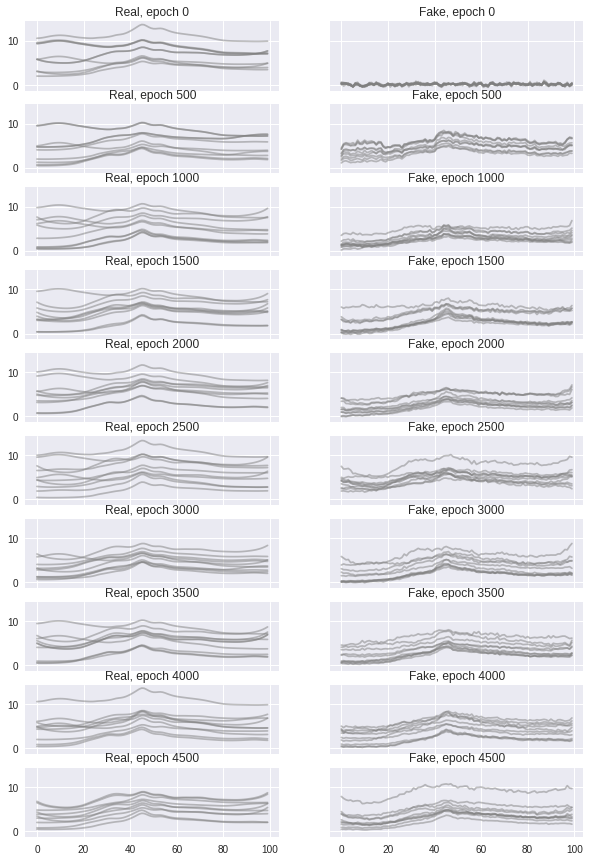
\includegraphics[width=17cm,height=15cm,keepaspectratio]{images/GAN_train.png}
\caption{Data generation process using GANs}
\label{fig:GANs train augmentation}
\end{center}
\end{figure}


\chapter{Deep learning model without augmentation}
\begin{figure}[ht]
	\begin{center}
		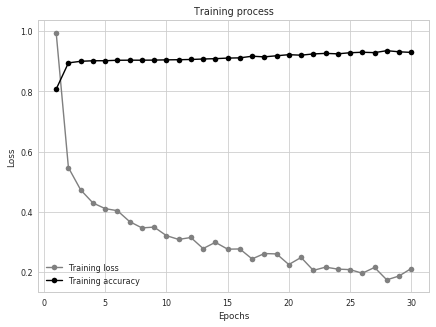
\includegraphics[width=12cm,height=10cm,keepaspectratio]{images/model1_training.png}
		\caption{Deep learning model without augmentation training process}
		\label{fig:first model training}
	\end{center}
\end{figure}

\chapter{Deep learning model training}
\begin{figure}[ht]
	\begin{center}
		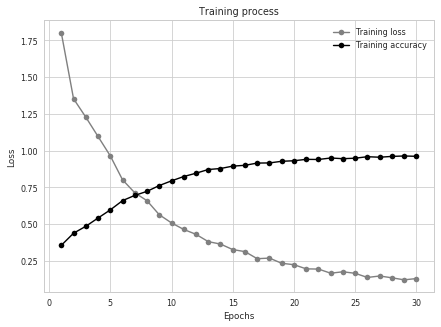
\includegraphics[width=\textwidth]{images/model_2.png}
		\caption{Training loss and accuracy for model with augmentation usign data-warping}
		\label{fig:second model}
	\end{center}
\end{figure}

\chapter{Deep learning model training}
\begin{figure}[ht]
	\begin{center}
		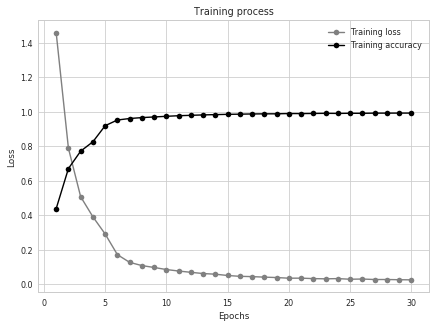
\includegraphics[width=\textwidth]{images/model_3.png}
		\caption{Training loss and accuracy for model with augmentation usign data-warping}
		\label{fig:third model}
	\end{center}
\end{figure}

\chapter{Model misclassification}
\begin{figure}[ht]
	\begin{center}
		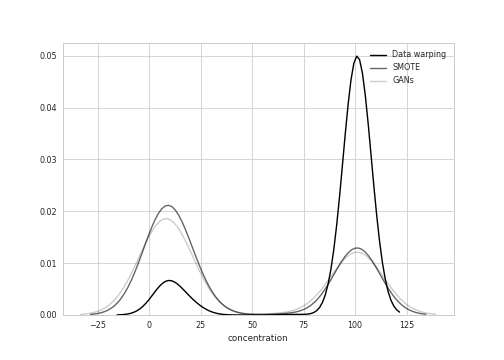
\includegraphics[width=\textwidth]{images/models_evaluation.png}
		\caption{Density plot of model missclassification at various concentration level }
		\label{fig:miss-classification}
	\end{center}
\end{figure}